%%%%%%%%%%%%%%%%%%%%%%%%%%%%%%%%%%%%%%%%%
% Beamer Presentation
% LaTeX Template
% Version 1.0 (10/11/12)
%
% This template has been downloaded from:
% http://www.LaTeXTemplates.com
%
% License:
% CC BY-NC-SA 3.0 (http://creativecommons.org/licenses/by-nc-sa/3.0/)
%
%%%%%%%%%%%%%%%%%%%%%%%%%%%%%%%%%%%%%%%%%

%----------------------------------------------------------------------------------------
%	PACKAGES AND THEMES
%----------------------------------------------------------------------------------------

\documentclass[aspectratio=169]{beamer}
\usepackage{listings}

\usepackage{color}
\usepackage{xcolor}
\usepackage{booktabs}
\usepackage{enumitem}

\definecolor{mygray}{rgb}{0.4,0.4,0.4}
\definecolor{myorange}{rgb}{1.0,0.4,0}
\newcommand{\gr}{\cellcolor{green!40}}
\newcommand{\rd}{\cellcolor{red!40}}

\lstset{
basicstyle=\tiny\sffamily\color{black},
commentstyle=\color{mygray},
frame=single,
keywordstyle=\color{blue},
showspaces=false,
showstringspaces=false,
stringstyle=\color{myorange},
tabsize=2,
language=C++
}


\mode<presentation> {

% The Beamer class comes with a number of default slide themes
% which change the colors and layouts of slides. Below this is a list
% of all the themes, uncomment each in turn to see what they look like.

%\usetheme{default}
%\usetheme{AnnArbor}
%\usetheme{Antibes}
%\usetheme{Bergen}
%\usetheme{Berkeley}
%\usetheme{Berlin}
%\usetheme{Boadilla}
\usetheme{CambridgeUS}
%\usetheme{Copenhagen}
%\usetheme{Darmstadt}
%\usetheme{Dresden}
%\usetheme{Frankfurt}
%\usetheme{Goettingen}
%\usetheme{Hannover}
%\usetheme{Ilmenau}
%\usetheme{JuanLesPins}
%\usetheme{Luebeck}
%\usetheme{Madrid}
%\usetheme{Malmoe}
%\usetheme{Marburg}
%\usetheme{Montpellier}
%\usetheme{PaloAlto}
%\usetheme{Pittsburgh}
%\usetheme{Rochester}
%\usetheme{Singapore}
%\usetheme{Szeged}
%\usetheme{Warsaw}

% As well as themes, the Beamer class has a number of color themes
% for any slide theme. Uncomment each of these in turn to see how it
% changes the colors of your current slide theme.

%\usecolortheme{albatross}
%\usecolortheme{beaver}
%\usecolortheme{beetle}
%\usecolortheme{crane}
%\usecolortheme{dolphin}
%\usecolortheme{dove}
%\usecolortheme{fly}
%\usecolortheme{lily}
%\usecolortheme{orchid}
%\usecolortheme{rose}
%\usecolortheme{seagull}
%\usecolortheme{seahorse}
%\usecolortheme{whale}
%\usecolortheme{wolverine}

%\setbeamertemplate{footline} % To remove the footer line in all slides uncomment this line
%\setbeamertemplate{footline}[page number] % To replace the footer line in all slides with a simple slide count uncomment this line

\setbeamertemplate{navigation symbols}{} % To remove the navigation symbols from the bottom of all slides uncomment this line
}
\setbeamercovered{transparent}
\setbeamersize{text margin left=30pt,text margin right=30pt} 


\usepackage[utf8]{inputenc}
\usepackage{graphicx} % Allows including images
\usepackage{booktabs} % Allows the use of \toprule, \midrule and \bottomrule in tables

\setitemize{label=\usebeamerfont*{itemize item}%
  \usebeamercolor[fg]{itemize item}
  \usebeamertemplate{itemize item}}

\setlist[description]{leftmargin=\parindent, labelindent=\parindent}

%----------------------------------------------------------------------------------------
%	TITLE PAGE
%----------------------------------------------------------------------------------------

\title[Randomness Testing Toolkit]{The automated testing of randomness with multiple statistical batteries} % The short title appears at the bottom of every slide, the full title is only on the title page

\author[lubomir.obratil@gmail.com]{Ľubomír Obrátil\\lubomir.obratil@gmail.com} % Your name
\date{22. 6. 2017} % Date, can be changed to a custom date

% Eliminates margins
\def\nomar{\list{}{\rightmargin-30pt \leftmargin-30pt}\item[]}
\let\endnomar=\endlist

\usepackage{makecell}
\usepackage{xcolor, colortbl}

\renewcommand\theadfont{\bfseries}

\begin{document}
%%%%%%%%%%%%%%%%%%%%%%%%%%%%%%%%%%%%%%%%%%%%%%%%%%%%%%%%%%%%%%%%%%%%%%%%%%%%%%%%%%%%%%%
%%%%%%%%%%%%%%%%%%%%%%%%%%%%%%%%% Presentation slides %%%%%%%%%%%%%%%%%%%%%%%%%%%%%%%%%
%%%%%%%%%%%%%%%%%%%%%%%%%%%%%%%%%%%%%%%%%%%%%%%%%%%%%%%%%%%%%%%%%%%%%%%%%%%%%%%%%%%%%%%
\begin{frame}
\titlepage % Print the title page as the first slide
\end{frame}

%%%%%%%%%%%%%%%%%%%%%%%%%%%%%%%%%%%%
% Overview of the thesis structure %
%%%%%%%%%%%%%%%%%%%%%%%%%%%%%%%%%%%%
\begin{frame}
\frametitle{Thesis structure}

\begin{itemize}
\item Creation of a unified interface supporting multiple statistical batteries.
\begin{itemize}
\item NIST Statistical Testing Suite
\item Dieharder
\item TestU01
\end{itemize}
\item Conducting the baseline (control) experiment to create a reference point for the further experiments.
\item Evaluating randomness of outputs of well-known cryptographic primitives.
\item Analysing validity of the Dieharder battery results.
\end{itemize}

\end{frame}

%%%%%%%%%%%%%%%%%%%%%%%%%%%%%%%%%%%%%%%
% Randomness Testing Toolkit overview %
%%%%%%%%%%%%%%%%%%%%%%%%%%%%%%%%%%%%%%%
\begin{frame}
\frametitle{Randomness Testing Toolkit -- overview}
\begin{itemize}
\item Design and implementation of a tool for consistent randomness evaluation.
\item Intended to be used by users without prior knowledge about statistical testing as well as by researchers in CRoCS. 
\item The developed tool (RTT) acts as an interface between the user and the statistical batteries -- common format of the battery settings and results.
\item The toolkit supports multiple statistical batteries -- NIST STS, Dieharder, and TestU01; it is possible to add more batteries over time.
\item Both standalone program and online service were developed.
\end{itemize}
\end{frame}

\begin{frame}
\frametitle{Randomness Testing Toolkit -- local interface}
\begin{nomar}
\centering
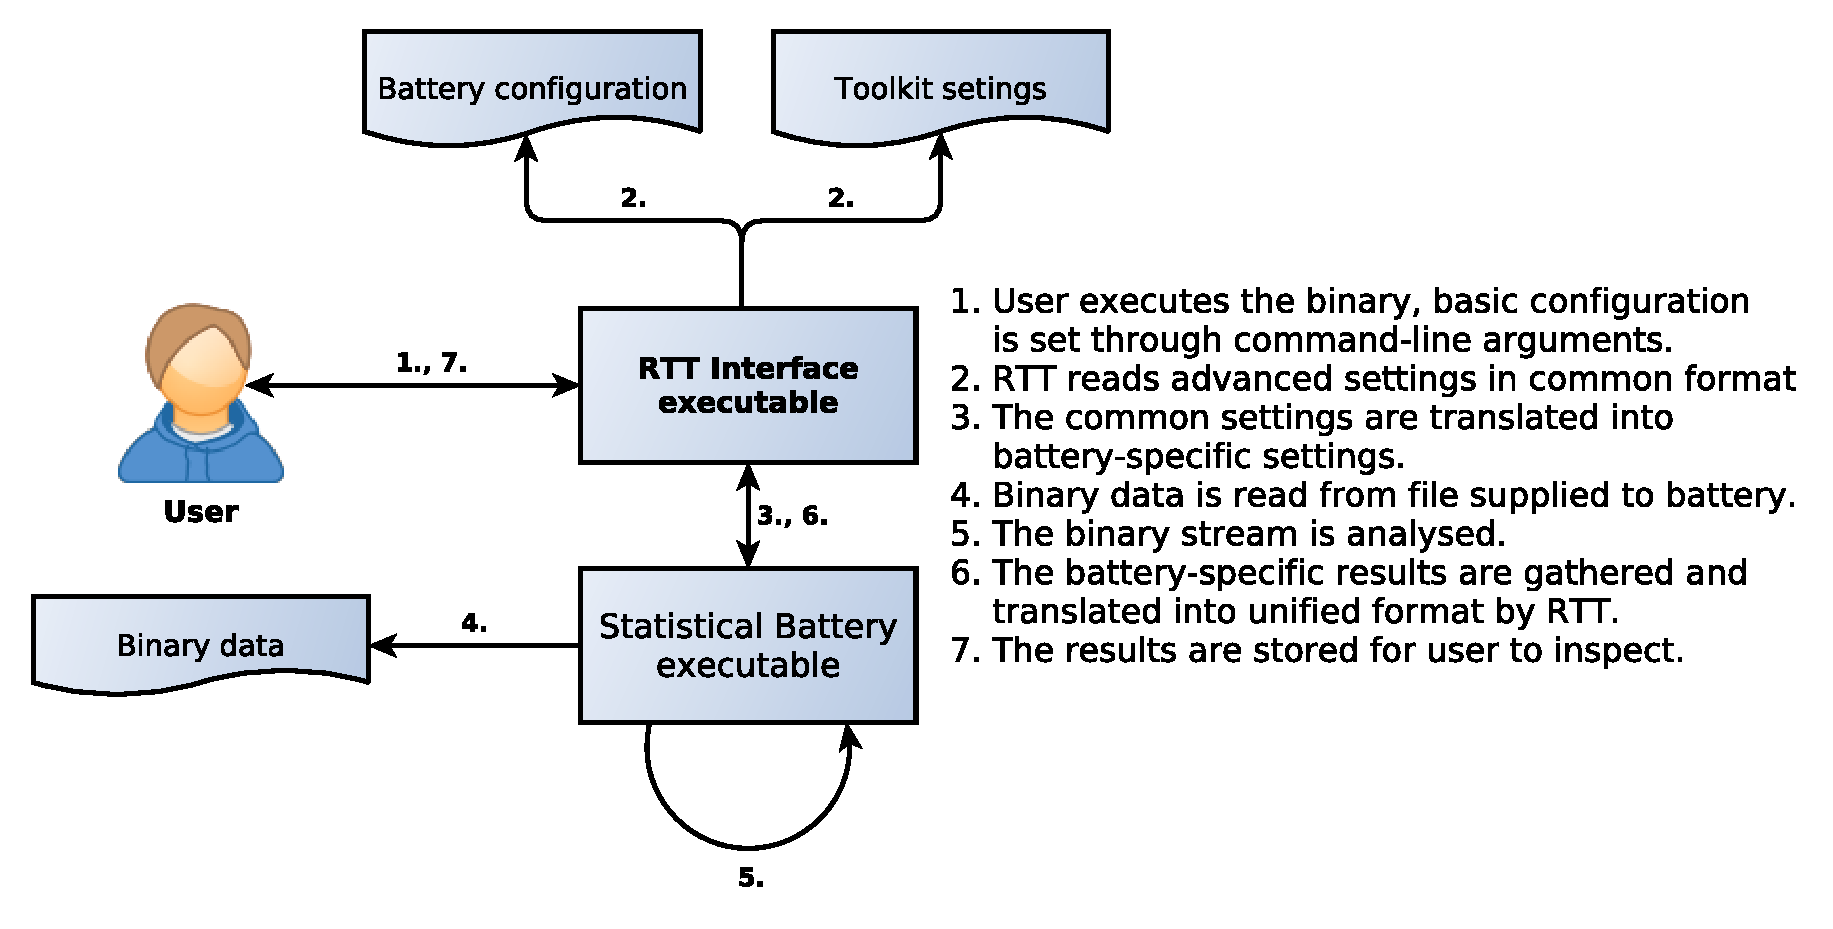
\includegraphics[width=\textwidth]{figures/local-rtt-workflow.pdf} 
\end{nomar}
\end{frame}

\begin{frame}
\frametitle{Randomness Testing Toolkit -- web service}
\begin{nomar}
\centering
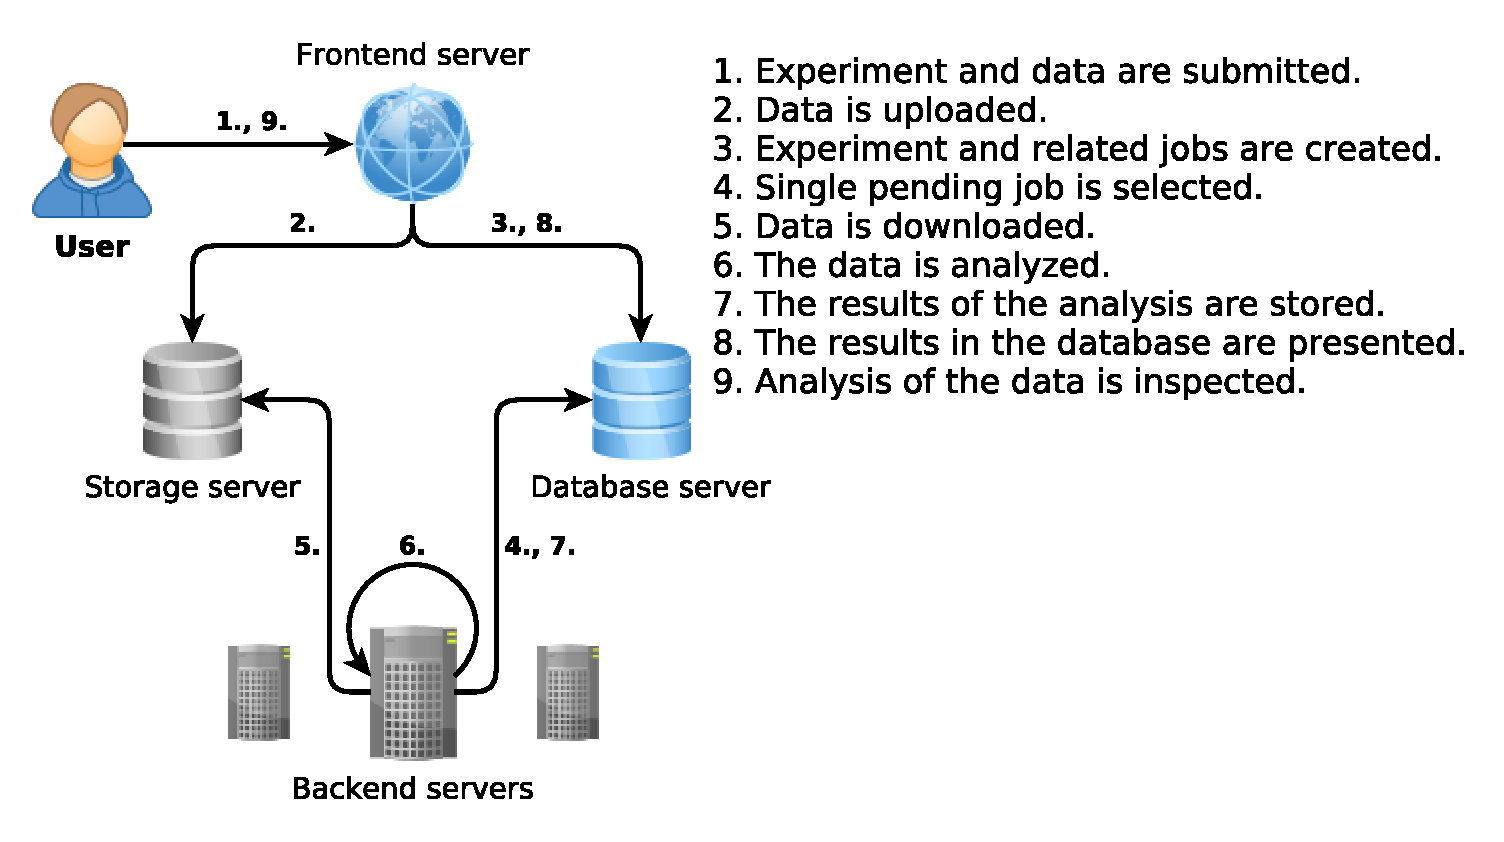
\includegraphics[width=.9\textwidth]{figures/rtt-ecosystem.pdf} 
\end{nomar}
\end{frame}

%%%%%%%%%%%%%%%%%%%%%%%%%%%%%%%%
% Statistical testing overview %
%%%%%%%%%%%%%%%%%%%%%%%%%%%%%%%%
\begin{frame}
\frametitle{Statistical testing of randomness -- 1/2}

\begin{description}
\item[Testing hypothesis -- $H_0$] \hfill \\
During the experiments, we evaluated the hypothesis that the analysed data were
produced by a truly random generator. We denote the hypothesis as $H_0$ (null hypothesis).
\item[Statistical battery] \hfill \\
Software with the purpose of detecting biases in data stream; collection of statistical tests.
\item[Statistical test] \hfill \\
A single unit in a statistical battery checking some property of the data (e.g. count of ones). Output of a test is the probability that the analysed data were produced by TRNG. Each test in a given battery will either fail ($H_0$ rejection) or pass ($H_0$ retainment).
\end{description}

\end{frame}

\begin{frame}
\frametitle{Statistical testing of randomness -- 2/2}

\begin{description}
\item[Significance level -- $\alpha$] \hfill \\
The significance level is set prior to the experiments (usually 0.001) and based on it, the null hypothesis is rejected or retained.
\item[False positive (Type I error)] \hfill \\
The false positive result is observed when $H_0$ holds true, but it is rejected -- stream
produced by TRNG is evaluated as non-random. The probability of Type I error is $\alpha$.
\item[False negative (Type II error)] \hfill \\
The false negative result is observed when $H_0$ is false, but it is not rejected -- stream generated by biased generator is evaluated as random.
\end{description}
\end{frame}

%%%%%%%%%%%%%%%%%%%%%%%
% Baseline experiment %
%%%%%%%%%%%%%%%%%%%%%%%
\begin{frame}
\frametitle{Establishing baseline results}
\begin{itemize}
\item The result of a battery is obtained from the proportion of the failed tests in the battery (e.g. we consider the data biased if more than 2 out of 15 tests fail). However, even data generated by a perfect TRNG may fail some tests (false positives).
\item To identify the maximum count of failed tests (assuming that the $H_0$ holds) we processed 8 TB of data generated by a quantum random generator (control experiment). Further experiments were interpreted based on these results.
\item To make the result interpretation more straightforward, results of certain tests were grouped together. As a consequence, the counts of failed tests are closer to expected (theoretical) numbers and therefore more easy to evaluate.
\end{itemize}
\end{frame}

%%%%%%%%%%%%%%%%%%%%%%%%%%%%%
% Usable testbed experiment %
%%%%%%%%%%%%%%%%%%%%%%%%%%%%%
\begin{frame}
\frametitle{Analysis of well-known algoritms -- 1/2}
\textbf{Goal:} Evaluate randomness of the outputs of round-reduced cryptographic primitives and observe their security margins.
\vspace{.3cm}
\begin{itemize}
\item We analysed 15 algorithms in multiple configurations. In total, more than 80 data streams were processed. The algorithms were chosen based on their popularity (AES, DES, RC4, ...) or their success in crypto competitions eSTREAM and SHA3 (Rabbit, Keccak, Gr\o stl, ...).
\item The interpretation of the results was based on the baseline obtained in the previous experiment.
\item The results were compared to another randomness analysis approach developed in CRoCS (EACirc).
\end{itemize}
\end{frame}

\begin{frame}
\frametitle{Analysis of well-known algoritms -- 2/2}

\begin{description}
\item[Experiment results] \hfill \\
\begin{itemize}
\item \textbf{Comparison to EACirc:} The batteries supported by RTT perform as equally well or better than EACirc. This can be caused by many reasons, namely by data consumption (EACirc requires a lesser amount of data) or internal data representation.
\item \textbf{Security margins:} Majority of the analysed algorithms had the security margins higher than 80\%. Even with a considerable increase in the performance of the statistical tools, the biases in full versions of the algorithms would go undetected.
\item \textbf{Biased outputs of full algorithms:} Statistical bias was detected in the outputs of the ciphers RC4 and Rabbit (winner of the eSTREAM competition). Compared to already published distinguishers our approach is easy and automated, but we assume zero IV and structured input data.
\end{itemize}
\end{description}

\end{frame}

%%%%%%%%%%%%%%%%%%%%%%%%%%%%%%
% Dieharder outputs analysis %
%%%%%%%%%%%%%%%%%%%%%%%%%%%%%%
\begin{frame}
\frametitle{Analysis of the results of Dieharder battery -- 1/2}
\textbf{Goal:} Verifying uniformity of partial results of Dieharder battery.

\begin{itemize}
\item Partial results of the battery are expected to be uniformly distributed on the interval $(0,1]$ during random data analysis; the assumption of uniformity is used to further process the battery results.
\item To verify this hypothesis, 8 TB of random data were processed by each test (110 tests in total). More than a billion of partial results was extracted and analysed.
\end{itemize}
\textbf{Experiment results}
\begin{itemize}
\item Out of 110 partial result sets, we found that 39 sets were not uniformly distributed.
\item The broken assumption can cause wrong result interpretation.
\item Further implications of the non-uniformity are a part of ongoing research.
\end{itemize}
\end{frame}

\begin{frame}
\frametitle{Analysis of the results of Dieharder battery -- 2/2}

\begin{figure}
\begin{nomar}
\centering
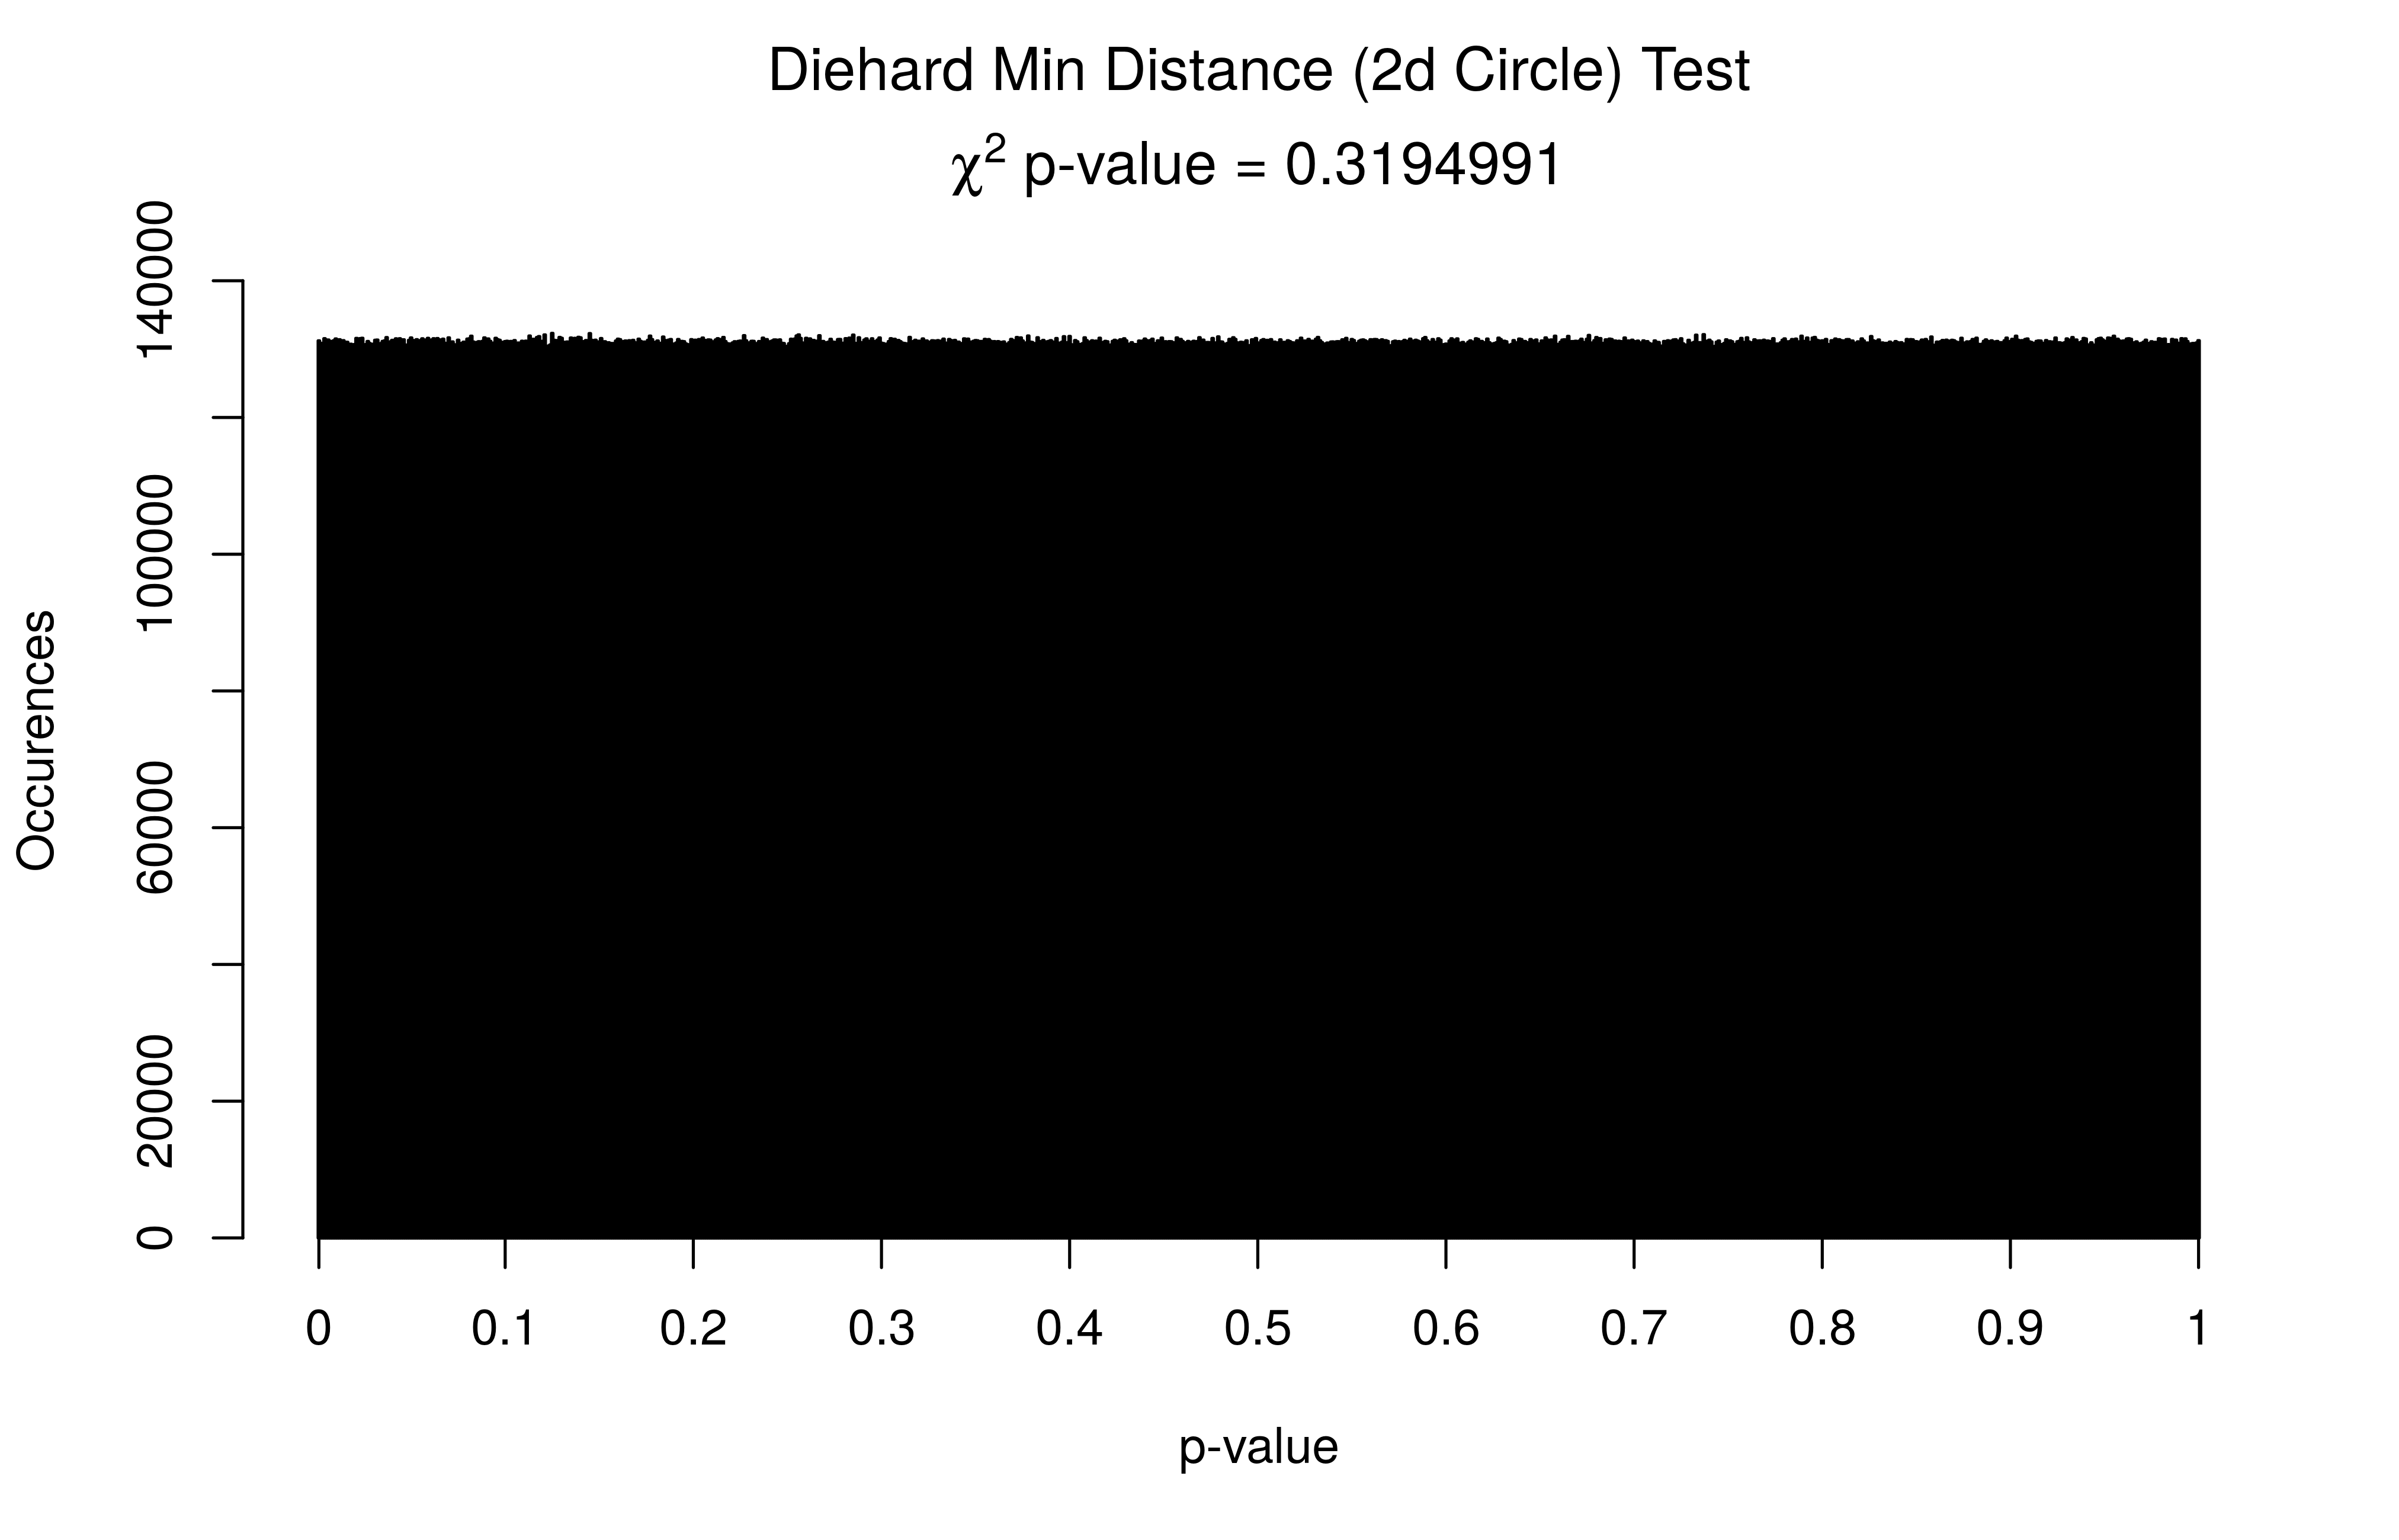
\includegraphics[width=.45\paperwidth]{figures/011.png} 
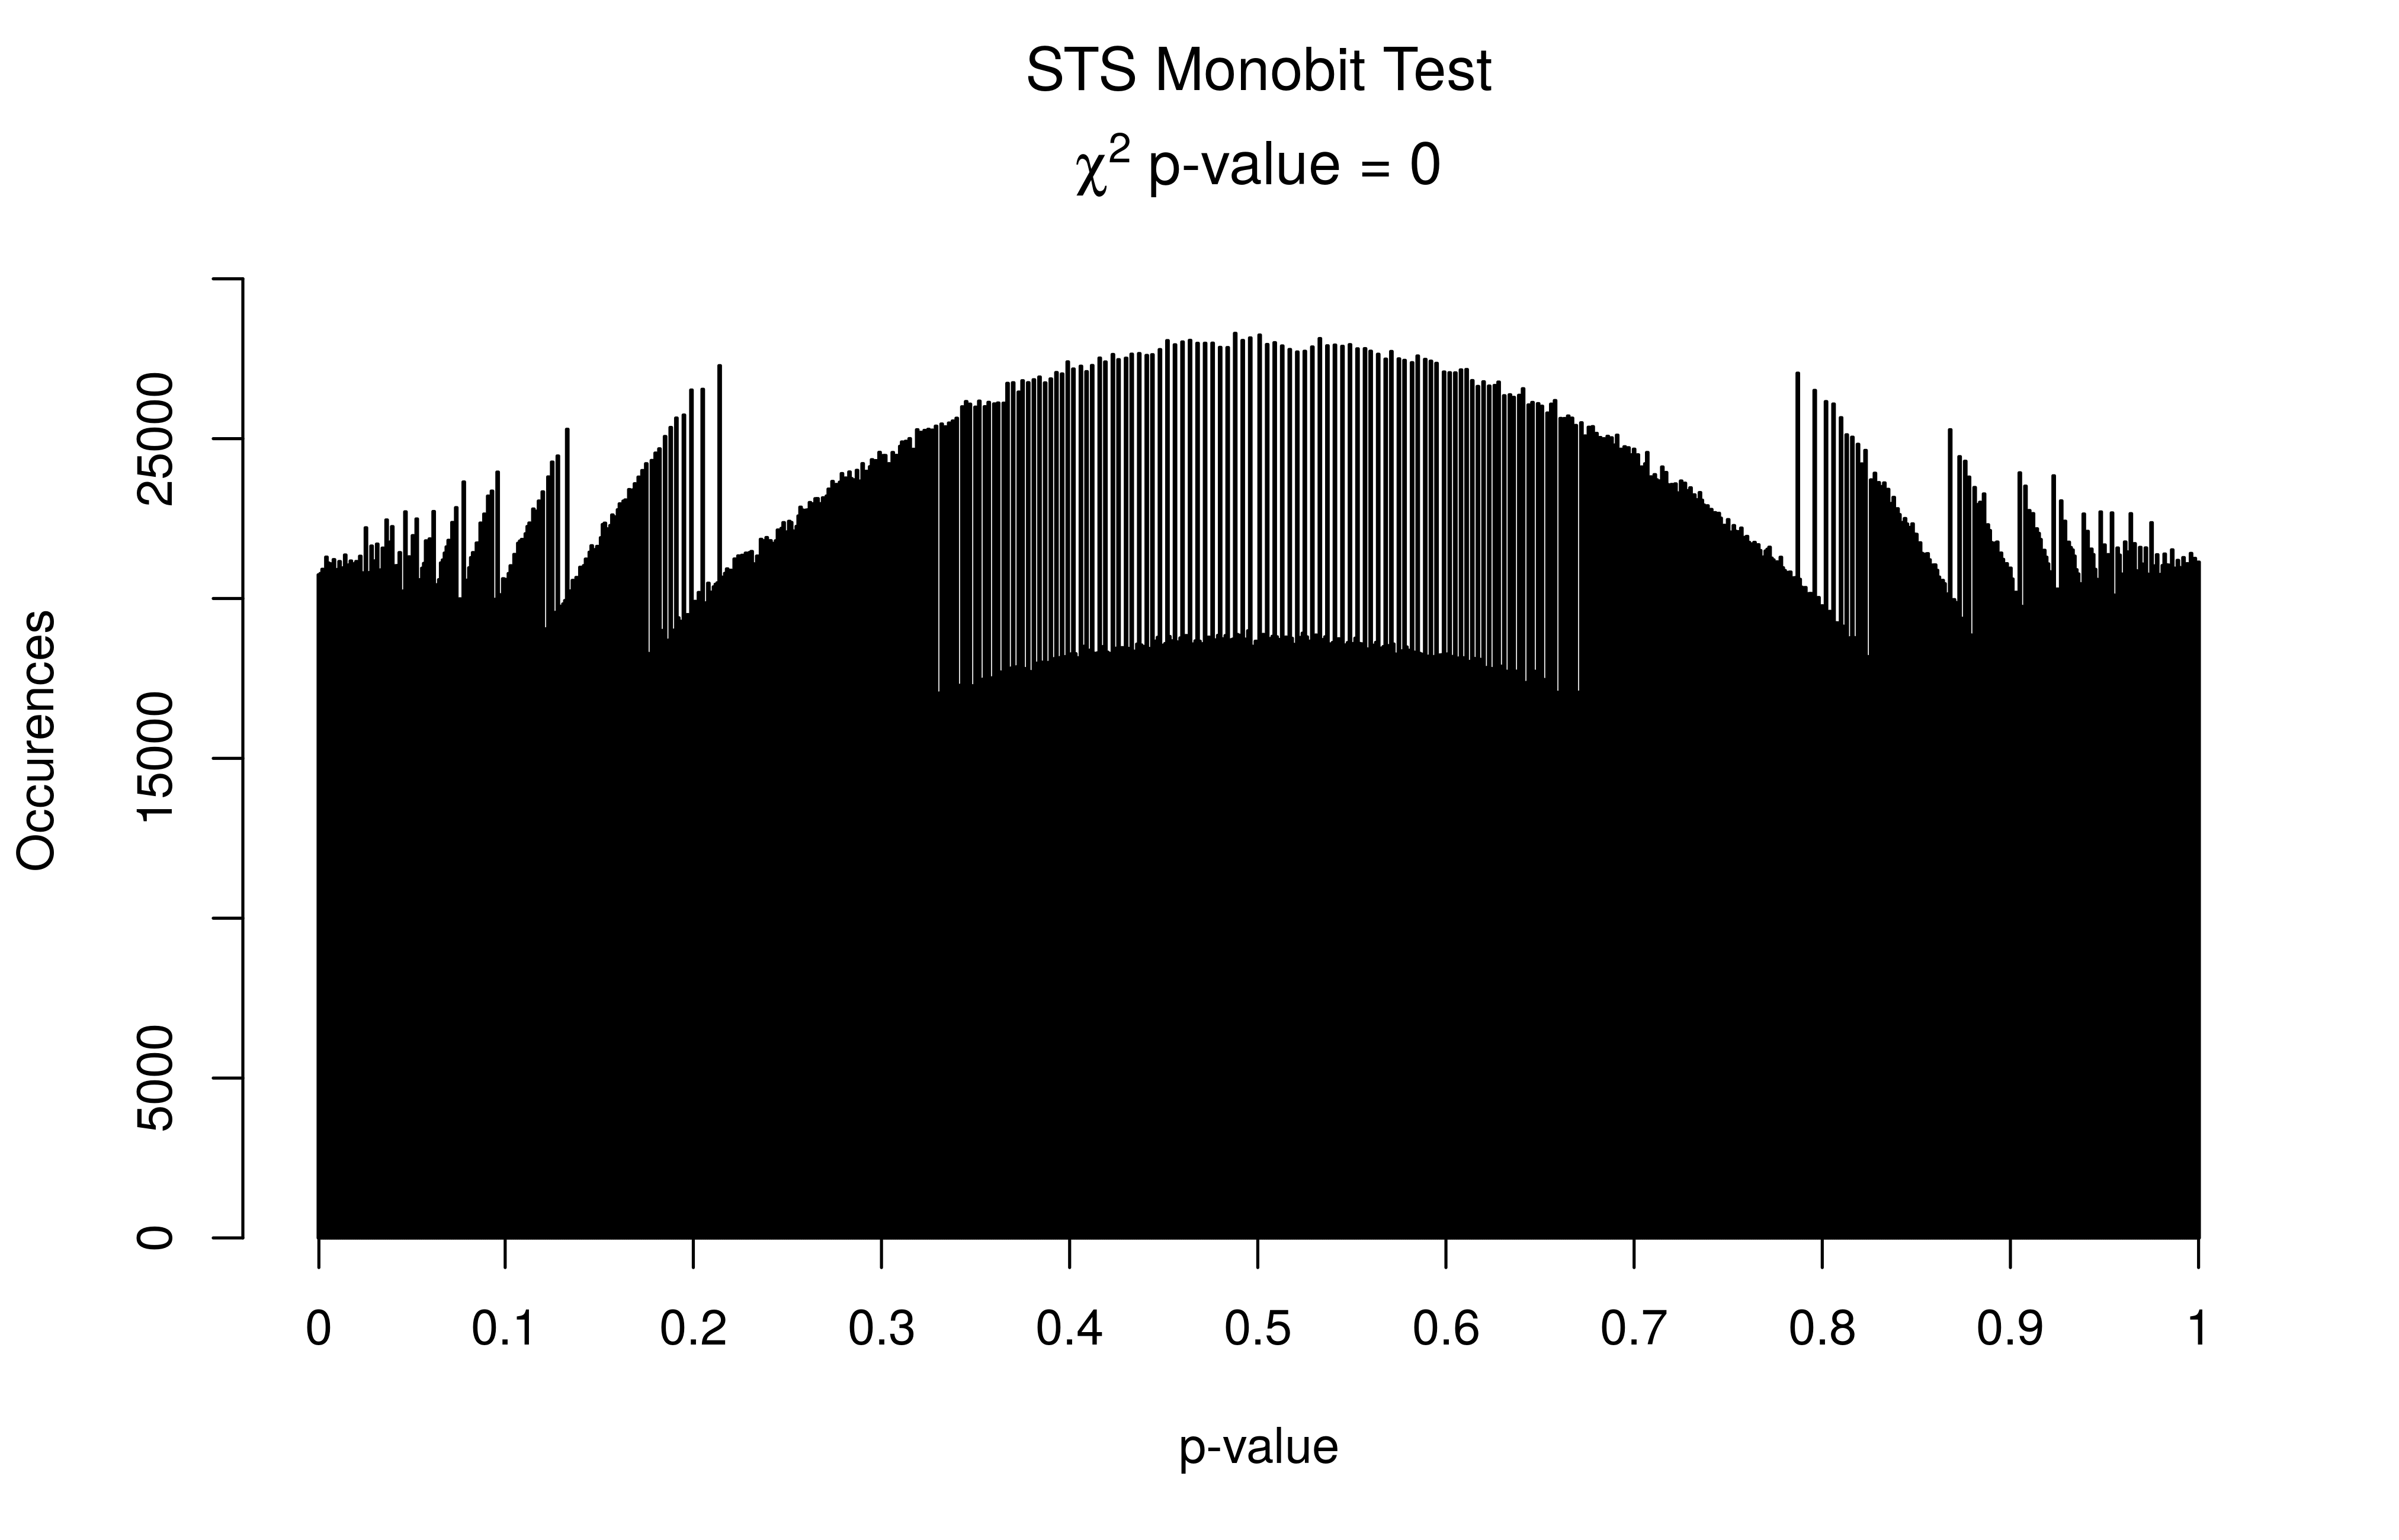
\includegraphics[width=.45\paperwidth]{figures/100.png}
\end{nomar}
\end{figure}

\end{frame}

%%%%%%%%%%%%%%%%%%%%%%%
% Last official frame %
%%%%%%%%%%%%%%%%%%%%%%%

\begin{frame}

\frametitle{References}
\begin{itemize}
\item \textbf{Randomness Testing Toolkit} \\ \url{https://github.com/crocs-muni/randomness-testing-toolkit}
\item \textbf{EACirc} \\ \url{https://github.com/crocs-muni/eacirc}
\item \textbf{NIST Statistical testing suite} \\ \url{http://csrc.nist.gov/groups/ST/toolkit/rng/documentation_software.html}
\item \textbf{Dieharder} \\ \url{http://www.phy.duke.edu/~rgb/General/dieharder.php}
\item \textbf{TestU01} \\ \url{http://simul.iro.umontreal.ca/testu01/tu01.html}
\end{itemize}

\end{frame}

%%%%%%%%%%%%%%%%%%%%%%%%%%%%%%%%%%%%%%%%%%%%%%%%%%%%%%%%%%%%%%%%%%%%%%%%%%%%%%%%%%%%%%%%
%%%%%%%%%%%%%%%%%%%%%%%%%%%% Additional details and figures %%%%%%%%%%%%%%%%%%%%%%%%%%%%
%%%%%%%%%%%%%%%%%%%%%%%%%%%%%%%%%%%%%%%%%%%%%%%%%%%%%%%%%%%%%%%%%%%%%%%%%%%%%%%%%%%%%%%%

%%%%%%%%%%%%%%%%%%%%%%%%%%%%%%
% Baseline experiment detail %
%%%%%%%%%%%%%%%%%%%%%%%%%%%%%%
\begin{frame}
\frametitle{Baseline experiment -- uncorrected results}
\begin{nomar}
\centering
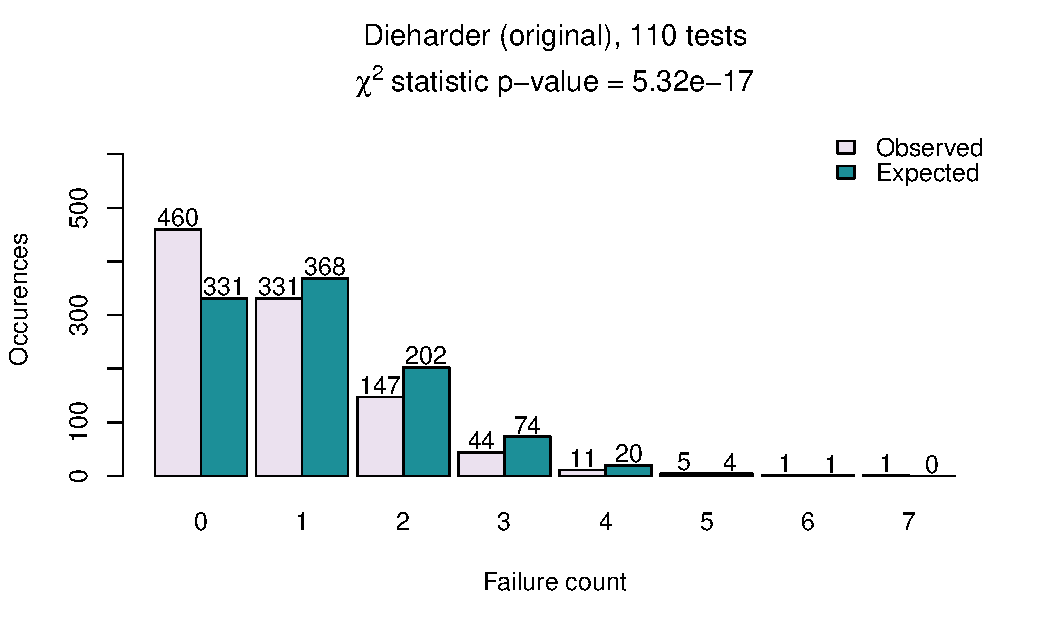
\includegraphics[width=.85\textwidth]{figures/dieharder-orig.pdf} 
\end{nomar}
\end{frame}

\begin{frame}
\frametitle{Baseline experiment -- corrected results}
\begin{nomar}
\centering
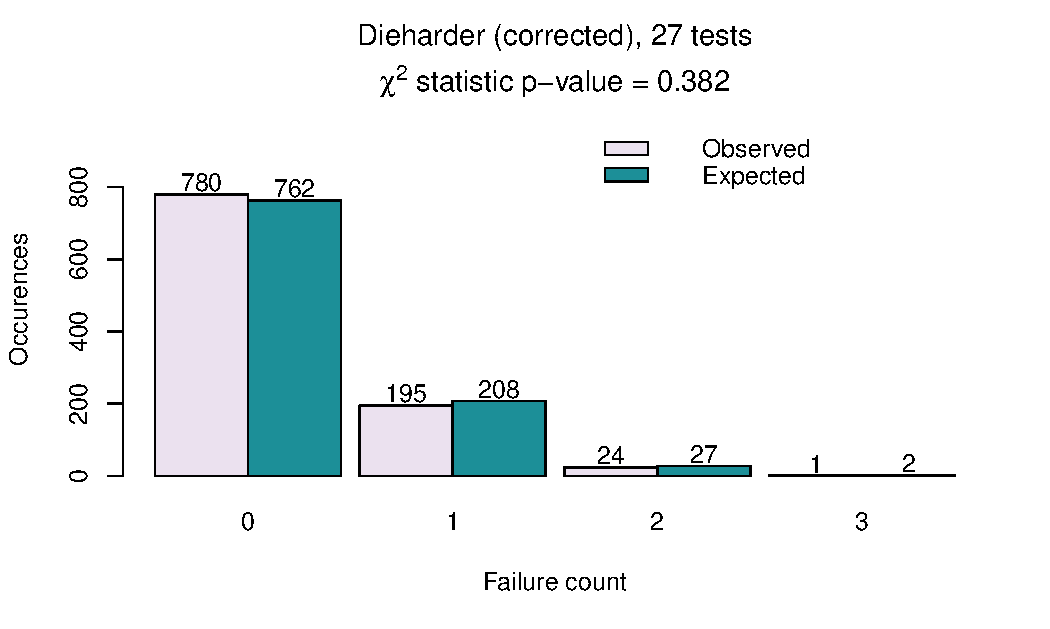
\includegraphics[width=.85\textwidth]{figures/dieharder-corr.pdf} 
\end{nomar}
\end{frame}

\begin{frame}
\frametitle{Baseline experiment -- reference failure counts}
\begin{table}
\begin{nomar}
\centering
\begin{tabular}{@{}lrrr@{}}
                                                                                                                  \toprule
                      & \multicolumn{2}{c}{\textbf{Closeness to expected results}} &                           \\ \cmidrule(lr){2-3}
\textbf{Battery name} & Uncorrected               & Uncorrected                    & \textbf{Allowed failures} \\ \midrule
Dieharder             &    $5.32 \cdot 10^{-17}$  & \gr$0.38$                      & 3/27                      \\ 
NIST STS              & \gr$2.17 \cdot 10^{-2}$   &    $4.44 \cdot 10^{-7}$        & 2/15                      \\ 
TU01 Small Crush      &    $0.71$                 & \gr$0.95$                      & 2/10                      \\ 
TU01 Crush            &    $3.36 \cdot 10^{-11}$  & \gr$3.31 \cdot 10^{-3}$        & 3/32                      \\ 
TU01 Rabbit           & \gr$2.02 \cdot 10^{-5}$   &    $1.45 \cdot 10^{-23}$       & 2/16                      \\ 
TU01 Alphabit         &    $2.14 \cdot 10^{-8}$   & \gr$2.8 \cdot 10^{-7}$         & 1/4                       \\ 
TU01 Block Alphabit   &    $1.87 \cdot 10^{-68}$  & \gr$5.15 \cdot 10^{-47}$       & 1/4                       \\ \bottomrule
\end{tabular}
\end{nomar}
\end{table}
\end{frame}

%%%%%%%%%%%%%%%%%%%%%%%%%%%%%%%%%
% Usable testbed results detail %
%%%%%%%%%%%%%%%%%%%%%%%%%%%%%%%%%
\begin{frame}
\frametitle{Analysis of well-known algorithms -- results}

\begin{table}
\begin{nomar}
\centering
\scalebox{0.75} {
\begin{tabular}{@{}lrrrr@{}}
                                                                                                                           \toprule
                   & \multicolumn{2}{c}{\textbf{Top biased round}} &                                                    \\ \cmidrule(lr){2-3}                       
\textbf{Algorithm} & RTT                & EACirc                   & \textbf{Total rounds} & \textbf{Security margin}   \\ \midrule
AES                &    3               & 3                        & 10                    &     7 rounds (70\%)        \\
BLAKE              &    1               & 1                        & 16                    &    15 rounds (94\%)        \\
Grain              & \gr6               & 2                        & 13                    &     7 rounds (54\%)        \\
Gr\o stl           &    2               & 2                        & 14                    &    12 rounds (86\%)        \\
JH                 &    6               & 6                        & 42                    &    36 rounds (86\%)        \\
Keccak             & \gr3               & 2                        & 24                    &    21 rounds (88\%)        \\
MD6                & \gr10              & 8                        & 104                   &    94 rounds (90\%)        \\
Rabbit             & \gr4               & 0                        & 4                     & \rd 0 rounds (0\%)         \\
RC4                & \gr--              & --                       & --                    & \rd 0 rounds (0\%)         \\
Salsa20            &    2               & 2                        & 20                    &    18 rounds (90\%)        \\
Single DES         & \gr5               & 4                        & 16                    &    11 rounds (69\%)        \\
Skein              & \gr4               & 3                        & 72                    &    68 rounds (94\%)        \\
SOSEMANUK          &    4               & 4                        & 25                    &    21 rounds (84\%)        \\
TEA                & \gr5               & 4                        & 32                    &    27 rounds (84\%)        \\
Triple DES         & \gr3               & 2                        & 16                    &    13 rounds (81\%)        \\ \bottomrule
\end{tabular}
}
\end{nomar}
\end{table}
\end{frame}

\end{document}
